%!TEX program = xelatex
%!TEX root = ../all_beamer.tex

%% !TEX root = all_beamer.tex
% ==============================================================================
% HEADER LATEX PER PRESENTAZIONI BEAMER
% Corso di Machine Learning - Giorgio Gambosi
% Università di Roma "Tor Vergata"
% ==============================================================================

% ------------------------------------------------------------------------------
% CLASSE DOCUMENTO E METADATI
% ------------------------------------------------------------------------------
\documentclass[aspectratio=169, 10pt]{beamer}

\subtitle{Course of Machine Learning}
\author{Giorgio Gambosi}
\institute[Tor Vergata]{Master's Degree in Computer Science\\University of Rome ``Tor Vergata''}
\date{A.Y. 2025--2026}

% ------------------------------------------------------------------------------
% PACCHETTI MATEMATICI
% ------------------------------------------------------------------------------
\usepackage{amsmath, amssymb, amsfonts, mathtools, amsthm}
\usepackage{bm}              % Simboli matematici in grassetto
\usepackage{upgreek}         % Lettere greche dritte
\usepackage{derivative}      % Gestione semplificata delle derivate

% ------------------------------------------------------------------------------
% PACCHETTI GRAFICI E VISUALIZZAZIONE
% ------------------------------------------------------------------------------
\usepackage{graphicx}        % Inclusione immagini
\usepackage{xcolor}          % Gestione colori
\usepackage{xkcdcolors}      % Colori aggiuntivi stile xkcd
\usepackage{microtype}       % Miglioramenti tipografici

% ------------------------------------------------------------------------------
% PACCHETTI PER TABELLE
% ------------------------------------------------------------------------------
\usepackage{booktabs}        % Tabelle professionali
\usepackage{array}           % Estensioni per tabelle
\usepackage{multirow}        % Celle multi-riga
\usepackage{multicol}        % Layout multi-colonna

% ------------------------------------------------------------------------------
% TIKZ E PGFPLOTS
% ------------------------------------------------------------------------------
\usepackage{tikz}
\usepackage{tikz-network}
\usepackage[customcolors]{hf-tikz}
\usepackage{pgfplots}
\pgfplotsset{compat=1.18}
\usepgfplotslibrary{fillbetween}

% Librerie TikZ
\usetikzlibrary{arrows, arrows.meta, decorations.pathmorphing, decorations.pathreplacing}
\usetikzlibrary{decorations.markings, snakes, positioning, backgrounds, fit, shadows}
\usetikzlibrary{automata, patterns, calc, intersections, through, shapes}
\usetikzlibrary{shapes.geometric, shapes.arrows, scopes, chains, matrix}

% ------------------------------------------------------------------------------
% ALTRI PACCHETTI
% ------------------------------------------------------------------------------
\usepackage[skins]{tcolorbox}  % Box colorati
\usepackage{subcaption}         % Sottocaption per figure
\usepackage{listings}           % Inclusione codice sorgente

% ------------------------------------------------------------------------------
% TEMA E STILE BEAMER
% ------------------------------------------------------------------------------
\usetheme{Madrid}
\usecolortheme{whale}
\useinnertheme{rounded}
\usefonttheme{professionalfonts}
\setbeamertemplate{navigation symbols}{}  % Rimuove simboli di navigazione

% ------------------------------------------------------------------------------
% DEFINIZIONE COLORI PERSONALIZZATI
% ------------------------------------------------------------------------------
% Colori principali del tema
\definecolor{MainBlue}{RGB}{31,56,100}      % Blu principale (header, titoli)
\definecolor{AccentBlue}{RGB}{70,130,180}   % Blu accento (blocchi)
\definecolor{AlertRed}{RGB}{160,30,30}      % Rosso per alert
\definecolor{ExGreen}{RGB}{30,120,60}       % Verde per esempi
\definecolor{BlockBg}{RGB}{220,232,246}     % Sfondo blocchi
\definecolor{torgray}{RGB}{220,225,235}     % Grigio Tor Vergata

% Colori alternativi (Tor Vergata style)
\definecolor{TvDark}{RGB}{30,50,80}         % Blu scuro header
\definecolor{TvMid}{RGB}{70,100,140}        % Blu medio blocchi
\definecolor{TvLight}{RGB}{210,220,235}     % Blu chiaro sfondi
\definecolor{TvAlert}{RGB}{160,30,30}       % Rosso alert
\definecolor{TvGreen}{RGB}{20,100,50}       % Verde esempi

% Colori supplementari
\definecolor{torred}{RGB}{153,0,0}
\definecolor{torcyan}{RGB}{0,112,192}
\definecolor{cerise}{HTML}{DA3A62}
\definecolor{teal}{HTML}{029386}
\definecolor{slateblue}{HTML}{5B5EA6}
\definecolor{orange}{HTML}{F97306}

% Colori per nodi TikZ
\definecolor{nodeblue}{RGB}{101,140,196}    % xkcd Faded Blue

% ------------------------------------------------------------------------------
% CONFIGURAZIONE COLORI BEAMER
% ------------------------------------------------------------------------------
\setbeamercolor{frametitle}{bg=MainBlue, fg=white}
\setbeamercolor{title}{bg=MainBlue, fg=white}
\setbeamercolor{structure}{fg=MainBlue}

% Blocchi standard
\setbeamercolor{block title}{bg=AccentBlue, fg=white}
\setbeamercolor{block body}{bg=BlockBg}

% Blocchi alert
\setbeamercolor{block title alerted}{bg=AlertRed, fg=white}
\setbeamercolor{block body alerted}{bg=red!8}

% Blocchi esempio
\setbeamercolor{block title example}{bg=ExGreen, fg=white}
\setbeamercolor{block body example}{bg=green!7}

% ------------------------------------------------------------------------------
% CONFIGURAZIONE FONT BEAMER
% ------------------------------------------------------------------------------
\setbeamerfont{frametitle}{size=\normalsize,series=\bfseries}
\setbeamerfont{block title}{size=\small,series=\bfseries}

% ------------------------------------------------------------------------------
% STILI TIKZ PERSONALIZZATI
% ------------------------------------------------------------------------------
\tikzset{
  >=latex,  % Frecce stile LaTeX di default
  % Nodi per reti neurali
  node/.style={thick,circle,draw=myblue,minimum size=22,inner sep=0.5,outer sep=0.6},
  node in/.style={node,green!20!black,draw=mygreen!30!black,fill=mygreen!25},
  node hidden/.style={node,blue!20!black,draw=myblue!30!black,fill=myblue!20},
  node convol/.style={node,orange!20!black,draw=myorange!30!black,fill=myorange!20},
  node out/.style={node,red!20!black,draw=myred!30!black,fill=myred!20},
  % Connessioni
  connect/.style={thick,mydarkblue},
  connect arrow/.style={-{Latex[length=4,width=3.5]},thick,mydarkblue,shorten <=0.5,shorten >=1},
  % Stili numerati per facile mappatura
  node 1/.style={node in},
  node 2/.style={node hidden},
  node 3/.style={node out}
}

% ------------------------------------------------------------------------------
% AMBIENTI TEOREMI
% ------------------------------------------------------------------------------
\setbeamertemplate{theorems}[numbered]
\newtheorem{mytheorem}{Theorem}
\newtheorem{mydefinition}{Definition}

% ------------------------------------------------------------------------------
% CONFIGURAZIONE LISTINGS (CODICE)
% ------------------------------------------------------------------------------
\lstset{
  language=Python,
  basicstyle=\ttfamily\tiny,
  keywordstyle=\color{MainBlue}\bfseries,
  commentstyle=\color{gray},
  frame=single,
  breaklines=true,
}

% ==============================================================================
% MACRO MATEMATICHE PERSONALIZZATE
% ==============================================================================

% ------------------------------------------------------------------------------
% SPAZI CALLIGRAFICI (Calligraphic spaces)
% ------------------------------------------------------------------------------
\providecommand{\calX}{\mathcal{X}}         % Spazio input
\providecommand{\calY}{\mathcal{Y}}         % Spazio output
\providecommand{\calH}{\mathcal{H}}         % Spazio ipotesi
\providecommand{\calT}{\mathcal{T}}         % Training set
\providecommand{\calA}{\mathcal{A}}         % Algoritmo
\providecommand{\calR}{\mathcal{R}}         % Rischio
\providecommand{\calF}{\mathcal{F}}         % Famiglia di funzioni
\providecommand{\calL}{\mathcal{L}}         % Loss function

% Alias per compatibilità
\providecommand{\Rr}{\mathcal{R}}
\providecommand{\Tr}{\mathcal{T}}
\providecommand{\Hr}{\mathcal{H}}

% ------------------------------------------------------------------------------
% RISCHIO E PROBABILITÀ
% ------------------------------------------------------------------------------
\providecommand{\barR}{\overline{\mathcal{R}}}  % Rischio empirico
\providecommand{\EmpR}{\overline{\mathcal{R}}}  % Rischio empirico (alias)
\providecommand{\Rbar}{\overline{\mathcal{R}}}  % Rischio empirico (alias)
\providecommand{\pM}{p_M}                       % Probabilità modello
\providecommand{\pC}{p_C}                       % Probabilità corretta
\providecommand{\Prob}[2]{\mathbb{P}_{#1}\!\left[#2\right]}  % Probabilità

% ------------------------------------------------------------------------------
% FUNZIONI INDICATRICI
% ------------------------------------------------------------------------------
\providecommand{\indicator}[1]{\mathbf{1}\!\left[#1\right]}  % Funzione indicatrice
\providecommand{\ind}[1]{\mathbf{1}[#1]}                      % Versione breve

% ------------------------------------------------------------------------------
% OPERATORI MATEMATICI
% ------------------------------------------------------------------------------
\providecommand{\argmax}{\operatorname*{arg\,max}}  % Argomento del massimo
\providecommand{\argmin}{\operatorname*{arg\,min}}  % Argomento del minimo
\providecommand{\vcd}[1]{\operatorname{VCdim}(#1)} % VC dimension
\providecommand{\defeq}{\stackrel{\text{def}}{=}}  % Definito come

% ------------------------------------------------------------------------------
% VETTORI E MATRICI (Bold Math)
% ------------------------------------------------------------------------------
% Vettori minuscoli
\providecommand{\bx}{\mathbf{x}}            % Vettore x
\providecommand{\bz}{\mathbf{z}}            % Vettore z
\providecommand{\bw}{\mathbf{w}}            % Vettore peso
\providecommand{\btt}{\mathbf{t}}           % Vettore target
\providecommand{\wvec}{\mathbf{w}}          % Vettore peso (alias)
\providecommand{\bth}{\boldsymbol{\theta}}  % Parametro theta

% Matrici maiuscole
\providecommand{\bX}{\mathbf{X}}            % Matrice dati
\providecommand{\bZ}{\mathbf{Z}}            % Matrice Z
\providecommand{\Xmat}{\mathbf{X}}          % Matrice dati (alias)
\providecommand{\Hmat}{\mathbf{H}}          % Matrice H
\providecommand{\Smat}{\mathbf{S}}          % Matrice scatter generica
\providecommand{\bS}{\mathbf{S}}            % Matrice scatter
\providecommand{\Ii}{\mathbf{I}}            % Matrice identità
\providecommand{\bZero}{\mathbf{0}}         % Vettore zero
\providecommand{\bPsi}{\boldsymbol{\Psi}}   % Matrice Psi

% Medie (overline)
\providecommand{\ox}{\overline{\mathbf{x}}} % Media vettore x
\providecommand{\ow}{\overline{\mathbf{w}}} % Media vettore w
\providecommand{\oX}{\overline{\mathbf{X}}} % Media matrice X

% Matrici scatter specifiche (analisi discriminante)
\providecommand{\SW}{\mathbf{S}_W}          % Within-class scatter
\providecommand{\SB}{\mathbf{S}_B}          % Between-class scatter
\providecommand{\ST}{\mathbf{S}_T}          % Total scatter
\providecommand{\GX}{G_{\mathbf{X}}}        % Matrice Gram

% ------------------------------------------------------------------------------
% COMANDI DI FORMATTAZIONE TESTO
% ------------------------------------------------------------------------------
\providecommand{\term}[1]{\textbf{\color{accent}#1}}        % Termine importante
\providecommand{\halert}[1]{{\color{AlertRed}\textbf{#1}}}  % Alert rosso
\providecommand{\mlalert}[1]{{\color{AccentBlue}\textbf{#1}}}  % Alert blu
\providecommand{\mlemph}[1]{{\color{MainBlue}\textit{#1}}}  % Enfasi blu

% ==============================================================================
% FINE HEADER
% ==============================================================================

\newcommand{\blankpage}{
\clearpage
\thispagestyle{empty}
\null
\clearpage
}

% ---------- Packages ----------

% ---------- Title ----------
\title[Foundations of ML]{Foundations of Machine Learning}

% ============================================================
%\begin{document}
% ============================================================

\begin{frame}[plain]
  \titlepage
\end{frame}

% ----------------------------------------
\begin{frame}{Outline}
  \tableofcontents
\end{frame}

% ============================================================
\section{Introduction}
% ============================================================

% -------- 1 --------
\begin{frame}{Introduction}{The fundamental observation}
  \begin{block}{Starting point}
    Real-world data contains \textcolor{AccentBlue}{\textbf{hidden patterns}} that reflect
    the process which generated it.
  \end{block}
  \bigskip
  \begin{itemize}
    \item Images, text, sensors, human behaviour: all exhibit \emph{regular structure}.
    \item Hidden patterns emerge from the \emph{generative process} underlying the data.
    \item The challenge of ML is to discover these patterns \textbf{automatically}, without
          being explicitly programmed with the governing rules.
    \item Discovery happens \textcolor{AccentBlue}{\textbf{by example}}: we start from a
          collection of observations, each a snapshot of the phenomenon we wish to understand.
  \end{itemize}
\end{frame}

% -------- 2 --------
\begin{frame}{Introduction}{Models and generalisation}
  \begin{itemize}
    \item From examples we build \textbf{models}: mathematical abstractions that capture
          relationships and patterns in the data.
    \item A model is a mathematical object (function, distribution, graph, \ldots) that
          summarises what we have learned.
    \item Models serve as tools for:
      \begin{itemize}
        \item Prediction on new, unseen data.
        \item Understanding the underlying phenomenon.
        \item Decision-making under uncertainty.
      \end{itemize}
    \item What matters is \emph{not} how well the model fits the training data,
          but how well it \textbf{generalises}.
  \end{itemize}
\end{frame}

% ============================================================
\section{The Three Learning Paradigms}
% ============================================================

% -------- 3 --------
\begin{frame}{The Three Learning Paradigms}{Overview}
  \begin{columns}[T]
    \column{0.32\textwidth}
    \begin{block}{Supervised}
      (Input, label) pairs.\\
      Learn the mapping $\x \to t$.
    \end{block}
    \column{0.32\textwidth}
    \begin{block}{Unsupervised}
      Inputs only, no labels.\\
      Explore intrinsic structure.
    \end{block}
    \column{0.32\textwidth}
    \begin{block}{Reinforcement}
      Agent + environment.\\
      Learn through rewards.
    \end{block}
  \end{columns}
  \bigskip
  \begin{itemize}
    \item Each paradigm poses distinct challenges and opportunities.
    \item This course focuses primarily on \textbf{supervised} and \textbf{unsupervised}
          learning.
  \end{itemize}
\end{frame}

% ============================================================
\section{Supervised Learning}
% ============================================================

% -------- 4 --------
\begin{frame}{Supervised Learning}{Definition and motivation}
  \begin{exampleblock}{Intuitive example}
    House dataset: area, rooms, location $\to$ selling price.
    We want to estimate the price of a \emph{new} house.
  \end{exampleblock}
  \bigskip
  \begin{itemize}
    \item Data consists of pairs $(\x_i, t_i)$: input features and corresponding target value.
    \item The goal is to learn the relationship $\x \to t$ so we can generalise to new inputs.
    \item The final model is either a function $h(\x)$ or a probability distribution
          $p(t|\x)$.
  \end{itemize}
\end{frame}

% -------- 5 --------
\begin{frame}{Supervised Learning}{Regression vs.\ Classification}
  \begin{columns}[T]
    \column{0.48\textwidth}
    \begin{block}{Regression}
      Target $t \in \mathbb{R}$ is continuous.
      \begin{itemize}
        \item House prices
        \item Future temperatures
        \item Stock values
        \item Drug dosages
      \end{itemize}
    \end{block}
    \column{0.48\textwidth}
    \begin{block}{Classification}
      Target $t \in \mathcal{Y}$ is categorical.
      \begin{itemize}
        \item Spam / not spam ($|\mathcal{Y}|=2$)
        \item Digits 0–9 ($|\mathcal{Y}|=10$)
        \item Medical diagnosis
        \item Text sentiment
      \end{itemize}
    \end{block}
  \end{columns}
  \bigskip
  \begin{itemize}
    \item \textcolor{AccentBlue}{\textbf{Binary}} classification: $|\mathcal{Y}| = 2$.
    \item \textcolor{AccentBlue}{\textbf{Multi-class}} classification: $|\mathcal{Y}| > 2$.
  \end{itemize}
\end{frame}

% ============================================================
\section{Unsupervised Learning}
% ============================================================

% -------- 6 --------
\begin{frame}{Unsupervised Learning}{Goals and main forms}
  \begin{itemize}
    \item \textbf{No labels available}: we explore the intrinsic structure of the data.
    \item \textbf{Clustering}: groups similar items without predefined categories; reveals
          natural segments.
    \item \textbf{Density estimation}: models $\pM(\x)$, the distribution that generated
          the data.
    \item \textbf{Dimensionality reduction}: projects high-dimensional data ($d \gg 1$) onto
          compact subspaces while preserving essential information.
  \end{itemize}
\end{frame}

% -------- 7 --------
\begin{frame}{Unsupervised Learning}{Generative modelling and further uses}
  \begin{itemize}
    \item \textcolor{AccentBlue}{\textbf{Generative modelling}}: learn to \emph{generate}
          new synthetic samples indistinguishable from real data.
      \begin{itemize}
        \item Large Language Models (LLM)
        \item Diffusion models (images, audio)
        \item Generative Adversarial Networks (GAN)
      \end{itemize}
    \item Requires having truly learned the deep structure of the data distribution.
  \end{itemize}
  \bigskip
  \begin{block}{Further applications}
    \begin{itemize}
      \item \textbf{Anomaly detection}: points that deviate from the learned pattern.
      \item \textbf{Visualisation}: 2D/3D projections of complex data.
      \item \textbf{Feature engineering}: richer, more informative representations.
    \end{itemize}
  \end{block}
\end{frame}

% ============================================================
\section{Reinforcement Learning}
% ============================================================

% -------- 8 --------
\begin{frame}{Reinforcement Learning}{The interaction paradigm}
  \begin{block}{Interaction cycle}
    \centering
    $s_t \xrightarrow{\;\pi\;} a_t \;\longrightarrow\; r_t,\, s_{t+1} \;\longrightarrow\; \cdots$
  \end{block}
  \begin{itemize}
    \item An \textcolor{AccentBlue}{\textbf{agent}} interacts sequentially with an
          environment.
    \item At each step it observes \textcolor{AccentBlue}{\textbf{state}} $s$, selects
          \textcolor{AccentBlue}{\textbf{action}} $a$, receives
          \textcolor{AccentBlue}{\textbf{reward}} $r$ and new state $s'$.
    \item The \textcolor{AccentBlue}{\textbf{policy}} $\pi: S \to A$ maps states to actions.
    \item Goal: find the optimal policy $\pi^*$ maximising the discounted cumulative reward:
      \[
        \pi^* = \argmax_{\pi}\; \mathbb{E}_{\pi}\!\left[\sum_{t=0}^{\infty} \gamma^t r_t\right],
        \qquad \gamma \in [0,1].
      \]
  \end{itemize}
\end{frame}

% -------- 9 --------
\begin{frame}{Reinforcement Learning}{Key tensions and applications}
  \begin{alertblock}{Fundamental tradeoff: exploration vs.\ exploitation}
    \begin{itemize}
      \item \textbf{Exploration}: try new actions to discover potentially better strategies.
      \item \textbf{Exploitation}: use known good actions to maximise immediate reward.
      \item Balancing both is essential for effective learning.
    \end{itemize}
  \end{alertblock}
  \bigskip
  \begin{block}{Successful applications}
    \begin{itemize}
      \item Games: AlphaGo defeated world Go champions.
      \item Robotics: learning motor skills and navigation.
      \item Autonomous systems: resource optimisation, scheduling.
    \end{itemize}
  \end{block}
\end{frame}

% ============================================================
\section{Data Representation}
% ============================================================

% -------- 10 --------
\begin{frame}{Data Representation}{The feature vector}
  \begin{block}{Definition}
    A \textcolor{AccentBlue}{\textbf{feature vector}} is
    $\x = (x_1, x_2, \ldots, x_d)$: a collection of $d$ numerical measurements describing
    one object. $d$ is called the \textcolor{AccentBlue}{\textbf{dimensionality}}.
  \end{block}
  \bigskip
  \begin{itemize}
    \item Real-world entities (images, documents, patients, transactions) must be converted
          into numerical vectors.
    \item Features are the \emph{raw material} from which models are built.
    \item The choice of features affects:
      \begin{itemize}
        \item Prediction quality.
        \item Computational efficiency of the learning algorithm.
        \item Generalisation ability of the model.
      \end{itemize}
  \end{itemize}
\end{frame}

% -------- 11 --------
\begin{frame}{Data Representation}{Examples of representations}
  \begin{columns}[T]
    \column{0.48\textwidth}
    \begin{exampleblock}{Images}
      \begin{itemize}
        \item Na\"ive: pixel intensity values (millions of features, noisy).
        \item Better: edge orientations, textures.
        \item Best: neural embeddings.
      \end{itemize}
    \end{exampleblock}
    \column{0.48\textwidth}
    \begin{exampleblock}{Text}
      \begin{itemize}
        \item Bag-of-words: word frequencies.
        \item TF-IDF: weighted relevance.
        \item Semantic embeddings (Word2Vec, BERT).
      \end{itemize}
    \end{exampleblock}
  \end{columns}
  \bigskip
  \begin{exampleblock}{Clinical data}
    Blood pressure, cholesterol, test results $\to$ vector of quantitative measurements.
  \end{exampleblock}
\end{frame}

% -------- 12 --------
\begin{frame}{Data Representation}{Feature Engineering}
  \begin{itemize}
    \item \textcolor{AccentBlue}{\textbf{Feature engineering}}: defining new features via
          functional combinations of existing ones, selecting the most informative subset,
          or learning entirely new representations.
    \item Often \emph{as important as} the choice of learning algorithm itself.
  \end{itemize}
  \bigskip
  \begin{columns}[T]
    \column{0.48\textwidth}
    \begin{block}{Expert-guided}
      A cardiologist knows which measurements matter for heart disease.
      Domain knowledge precedes data.
    \end{block}
    \column{0.48\textwidth}
    \begin{block}{Automated}
      Unsupervised learning techniques autonomously discover the most informative
      representations (e.g.\ autoencoders, PCA).
    \end{block}
  \end{columns}
\end{frame}

% ============================================================
\section{The Learning Process}
% ============================================================

% -------- 13 --------
\begin{frame}{The Learning Process}{From training to generalisation}
  \begin{itemize}
    \item We start from a \textcolor{AccentBlue}{\textbf{training set}}
          $\mathcal{T} = \{(\x_1, t_1), \ldots, (\x_n, t_n)\}$.
    \item The learning algorithm builds a model that captures the patterns present in
          $\mathcal{T}$.
    \item The crucial point: we do \emph{not} care how well the model fits the training data.
  \end{itemize}
  \bigskip
  \begin{alertblock}{The real objective: generalisation}
    We want the model to perform well on \textbf{new, unseen data} — sampled from the same
    process that generated the training set.
  \end{alertblock}
\end{frame}

% -------- 14 --------
\begin{frame}{The Learning Process}{Key concepts}
  \begin{itemize}
    \item \textbf{Capacity / Complexity}: how flexible the model is.
          Higher capacity can capture more intricate patterns, but risks overfitting.
    \item \textbf{Bias–variance tradeoff}: tension between underfitting (model too simple)
          and overfitting (model too adapted to training noise).
    \item \textbf{Regularisation}: techniques that penalise model complexity, encouraging
          simpler solutions that generalise better.
    \item \textbf{Generalisation}: the ability to transfer learned knowledge to new
          situations.
  \end{itemize}
\end{frame}

% -------- 15 --------
\begin{frame}{The Learning Process}{The role of models}
  \begin{itemize}
    \item Models are the bridge between data and prediction: they embody what we have
          learned from the training set.
    \item In \textbf{supervised} learning: the model captures the input–output relationship,
          enabling predictions on new inputs.
    \item In \textbf{unsupervised} learning: the model captures the structure of the data
          distribution.
    \item Possible forms of a model:
      \begin{itemize}
        \item Linear function.
        \item Deep neural network.
        \item Probabilistic distribution.
        \item Tree ensemble (e.g.\ Random Forest).
      \end{itemize}
    \item What unites them all: building from data something that \emph{transfers knowledge}
          to new situations.
  \end{itemize}
\end{frame}

% ============================================================
\section{Formal Definition}
% ============================================================

% -------- 16 --------
\begin{frame}{Formal Definition}{Domain set and Label set}
  \begin{columns}[T]
    \column{0.48\textwidth}
    \begin{block}{Domain set $\calX$}
      Set of objects we wish to label.
      \begin{itemize}
        \item Each $\x \in \calX$ is a vector of $d$ features.
        \item $\x = (x_1, \ldots, x_d)$;\; $d$ = dimensionality.
        \item More complex structures (sequences, graphs) are also possible.
      \end{itemize}
    \end{block}
    \column{0.48\textwidth}
    \begin{block}{Label set $\calY$}
      Set of possible output values.
      \begin{itemize}
        \item $\calY \subseteq \mathbb{R}$ (continuous) $\Rightarrow$ \textbf{regression}.
        \item $\calY$ finite $\Rightarrow$ \textbf{classification}.
        \item $|\calY|=2$: binary.
        \item $|\calY|>2$: multi-class.
      \end{itemize}
    \end{block}
  \end{columns}
\end{frame}

% -------- 17 --------
\begin{frame}{Formal Definition}{Training set and data structures}
  \begin{itemize}
    \item The learning algorithm $\calA$ receives a training set:
          $\calT = \{(\x_1, t_1), \ldots, (\x_n, t_n)\}$
    \item Organised as:
      \begin{itemize}
        \item \textcolor{AccentBlue}{\textbf{Feature matrix}} $\mathbf{X} \in \mathbb{R}^{n\times d}$:
              objects as rows.
        \item \textcolor{AccentBlue}{\textbf{Target vector}} $\mathbf{t} \in \calY^n$:
              corresponding labels.
      \end{itemize}
    \item Output of the algorithm: a
          \textcolor{AccentBlue}{\textbf{prediction rule}} $h : \calX \to \calY$
          (also called \emph{classifier} or \emph{regressor}).
  \end{itemize}
  \bigskip
  \begin{block}{Goal}
    $h$ must correctly predict label $y$ for any new object $\x$ it encounters.
  \end{block}
\end{frame}

% -------- 18 --------
\begin{frame}{Formal Definition}{Two output strategies}
  \begin{columns}[T]
    \column{0.48\textwidth}
    \begin{block}{Direct value prediction}
      $y = h(\x)$
      \begin{itemize}
        \item Single predicted label returned directly.
        \item Simple and computationally efficient.
        \item Does not quantify uncertainty.
      \end{itemize}
    \end{block}
    \column{0.48\textwidth}
    \begin{block}{Probability distribution}
      $p(y|\x)$ for each $y \in \calY$
      \begin{itemize}
        \item Estimates probability of each label.
        \item Richer: captures uncertainty.
        \item Final prediction via decision rule, e.g.\ $\hat y = \argmax_y p(y|\x)$.
      \end{itemize}
    \end{block}
  \end{columns}
\end{frame}

% ============================================================
\section{Three Approaches to Prediction}
% ============================================================

% -------- 19 --------
\begin{frame}{Three Approaches}{Overview}
  \begin{table}
    \centering
    \begin{tabular}{lll}
      \toprule
      \textbf{Approach} & \textbf{Core idea} & \textbf{Example}\\
      \midrule
      Direct prediction & Entire training set used at prediction time & $k$-NN\\
      Model-based       & Learn $h_\calT \in \calH$ during a training phase & Linear regression\\
      Ensemble          & Combine multiple weighted predictors & Random Forest\\
      \bottomrule
    \end{tabular}
  \end{table}
  \bigskip
  \begin{itemize}
    \item Three distinct philosophies about \emph{when} and \emph{how} to process the
          training data.
  \end{itemize}
\end{frame}

% -------- 20 --------
\begin{frame}{Approach 1: Direct Prediction}{Data-flow diagram}
  \begin{center}
  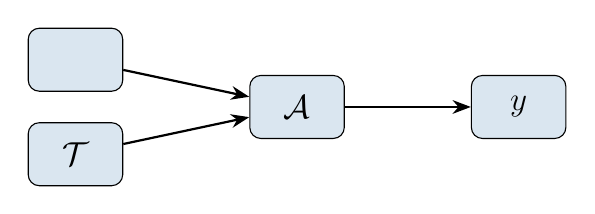
\begin{tikzpicture}[
    node distance=1.6cm,
    box/.style={draw, rounded corners, minimum width=1.2cm, minimum height=0.8cm,
                fill=AccentBlue!20, font=\large},
    arr/.style={-Stealth, thick}
  ]
    \node[box] (A)  {$\mathcal{A}$};
    \node[box, left=of A, yshift=0.6cm]  (x)  {$\x$};
    \node[box, left=of A, yshift=-0.6cm] (T)  {$\mathcal{T}$};
    \node[box, right=of A] (y)  {$y$};
    \draw[arr] (x) -- (A);
    \draw[arr] (T) -- (A);
    \draw[arr] (A) -- (y);
  \end{tikzpicture}
  \end{center}
  \begin{itemize}
    \item Both the new point $\x$ and the entire training set $\calT$ are inputs to the
          algorithm $\calA$ at prediction time.
    \item No separate learning phase; no compact model is built.
    \item All knowledge stays in the raw training examples.
  \end{itemize}
\end{frame}

% -------- 21 --------
\begin{frame}{Approach 1: Direct Prediction}{$k$-Nearest Neighbours}
  \begin{exampleblock}{kNN algorithm}
    To predict the class of a new point $\x$:
    \begin{enumerate}
      \item Find the $k$ training points closest to $\x$ under a distance metric
            (e.g.\ Euclidean).
      \item Predict the majority class among those $k$ neighbours.
    \end{enumerate}
  \end{exampleblock}
  \bigskip
  \begin{columns}[T]
    \column{0.48\textwidth}
    \begin{block}{Advantages}
      \begin{itemize}
        \item Flexible, locally adaptive.
        \item No training phase.
        \item Simple to implement.
      \end{itemize}
    \end{block}
    \column{0.48\textwidth}
    \begin{alertblock}{Disadvantages}
      \begin{itemize}
        \item Costly at prediction time: $\mathcal{O}(n)$.
        \item Must store entire $\calT$.
        \item Suffers from the \emph{curse of dimensionality}.
      \end{itemize}
    \end{alertblock}
  \end{columns}
\end{frame}

% -------- 22 --------
\begin{frame}{Approach 2: Model-Based Learning}{Data-flow diagram}
  \begin{center}
  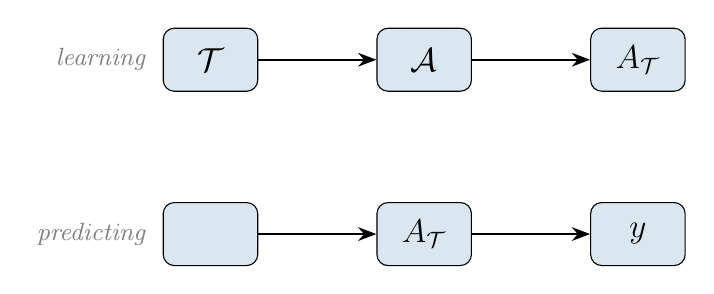
\begin{tikzpicture}[
    node distance=1.5cm,
    box/.style={draw, rounded corners, minimum width=1.2cm, minimum height=0.8cm,
                fill=AccentBlue!20, font=\large},
    arr/.style={-Stealth, thick},
    label/.style={font=\small\itshape, text=gray}
  ]
    % learning row
    \node[box] (T)  {$\mathcal{T}$};
    \node[box, right=of T] (A)  {$\mathcal{A}$};
    \node[box, right=of A] (AT) {$A_{\mathcal{T}}$};
    \draw[arr] (T) -- (A);
    \draw[arr] (A) -- (AT);
    \node[label, left=0.1cm of T] {learning};

    % predicting row
    \node[box, below=1.4cm of T] (x)   {$\x$};
    \node[box, right=1.5cm of x]  (AT2) {$A_{\mathcal{T}}$};
    \node[box, right=of AT2]       (y)   {$y$};
    \draw[arr] (x) -- (AT2);
    \draw[arr] (AT2) -- (y);
    \node[label, left=0.1cm of x] {predicting};
  \end{tikzpicture}
  \end{center}
  \begin{itemize}
    \item \textbf{Learning phase}: algorithm $\calA$ maps $\calT \to A_\calT$ (a fixed
          learned function).
    \item \textbf{Prediction phase}: $A_\calT$ maps new $\x \to y$ efficiently, with no
          access to $\calT$.
  \end{itemize}
\end{frame}

% -------- 23 --------
\begin{frame}{Approach 2: Model-Based Learning}{Hypothesis class}
  \begin{itemize}
    \item Define a \textcolor{AccentBlue}{\textbf{hypothesis class}} $\calH$: a predefined
          family of functions $h : \calX \to \calY$.
    \item The learning algorithm $\calA$ selects the function $h_\calT \in \calH$ that best
          explains the training data.
    \item Once $h_\calT$ is learned, prediction is immediate: $y = h_\calT(\x)$.
  \end{itemize}
  \bigskip
  \begin{block}{Parametric classes}
    Often $\calH = \calH_{\boldsymbol\theta}$: functions with the same structure but
    differing parameters.\\
    Learning $\equiv$ finding the optimal
    $\boldsymbol\theta^* = (\theta_1, \ldots, \theta_m)$.
  \end{block}
\end{frame}

% -------- 24 --------
\begin{frame}{Approach 2: Model-Based Learning}{Example: Linear Regression}
  \begin{exampleblock}{Linear regression}
    Assume the target is a linear combination of features:
    \[
      y = \sum_{i=1}^{d} w_i x_i + w_0 = \w^\top \bar{\x}
    \]
    where $\w = (w_0, w_1, \ldots, w_d)^\top$ and
    $\bar{\x} = (1, x_1, \ldots, x_d)^\top$.
  \end{exampleblock}
  \begin{itemize}
    \item $\calH$ = all $(d+1)$-dimensional linear functions.
    \item The algorithm finds weights $\w$ minimising prediction error on the training set.
    \item \textbf{Advantages}: efficient at prediction time ($\mathcal{O}(d)$),
          interpretable, compact.
  \end{itemize}
\end{frame}

% -------- 25 --------
\begin{frame}{Approach 3: Ensemble Learning}{Data-flow diagram}
  \begin{center}
  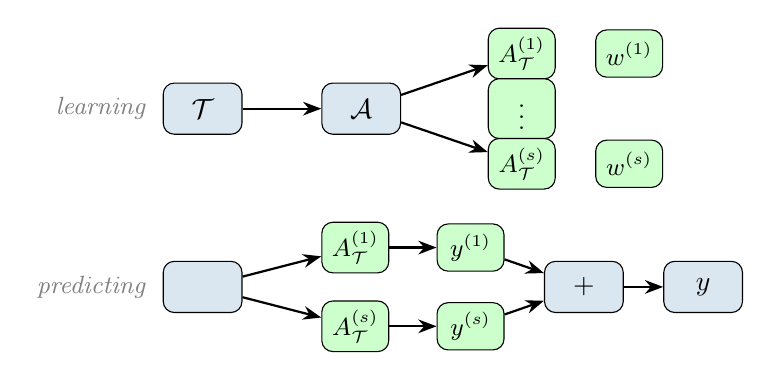
\begin{tikzpicture}[
    node distance=0.9cm and 1.1cm,
    box/.style={draw, rounded corners, minimum width=1.0cm, minimum height=0.65cm,
                fill=AccentBlue!20, font=\normalsize},
    sbox/.style={draw, rounded corners, minimum width=0.85cm, minimum height=0.6cm,
                 fill=green!20, font=\small},
    arr/.style={-Stealth, thick},
    label/.style={font=\small\itshape, text=gray}
  ]
    % learning
    \node[box] (T) {$\mathcal{T}$};
    \node[box, right=1.0cm of T] (A) {$\mathcal{A}$};
    \node[sbox, right=1.1cm of A, yshift= 0.7cm] (A1) {$A_\calT^{(1)}$};
    \node[sbox, right=1.1cm of A]                (Ad) {$\vdots$};
    \node[sbox, right=1.1cm of A, yshift=-0.7cm] (As) {$A_\calT^{(s)}$};
    \node[sbox, right=0.5cm of A1] (w1) {$w^{(1)}$};
    \node[sbox, right=0.5cm of As] (ws) {$w^{(s)}$};
    \draw[arr](T)--(A); \draw[arr](A)--(A1); \draw[arr](A)--(As);
    \node[label, left=0.1cm of T]{learning};

    % predicting
    \node[box, below=1.6cm of T] (x) {$\x$};
    \node[sbox, right=1.0cm of x, yshift= 0.5cm] (B1) {$A_\calT^{(1)}$};
    \node[sbox, right=1.0cm of x, yshift=-0.5cm] (Bs) {$A_\calT^{(s)}$};
    \node[sbox, right=0.6cm of B1] (y1) {$y^{(1)}$};
    \node[sbox, right=0.6cm of Bs] (ys) {$y^{(s)}$};
    \node[box,  right=0.5cm of y1, yshift=-0.5cm] (plus) {$+$};
    \node[box,  right=0.5cm of plus] (y) {$y$};
    \draw[arr](x)--(B1); \draw[arr](x)--(Bs);
    \draw[arr](B1)--(y1); \draw[arr](Bs)--(ys);
    \draw[arr](y1)--(plus); \draw[arr](ys)--(plus); \draw[arr](plus)--(y);
    \node[label, left=0.1cm of x]{predicting};
  \end{tikzpicture}
  \end{center}
\end{frame}

% -------- 26 --------
\begin{frame}{Approach 3: Ensemble Learning}{General principle}
  \begin{itemize}
    \item Rather than searching for a single best predictor, build $s$
          \textcolor{AccentBlue}{\textbf{predictors}} and combine their outputs.
    \item Predictors may differ in structure, parameters, or the subset of training data
          used.
    \item Each is assigned a weight $w^{(i)} \geq 0$ reflecting its estimated reliability,
          with $\sum_{i=1}^s w^{(i)} = 1$.
  \end{itemize}
  \bigskip
  \begin{block}{The three-stage process}
    \begin{enumerate}
      \item \textbf{Learning}: derive $h^{(1)}_\calT, \ldots, h^{(s)}_\calT$ from $\calT$.
      \item \textbf{Weighting}: assign weights $w^{(i)}$.
      \item \textbf{Combination}: aggregate predictions at test time.
    \end{enumerate}
  \end{block}
\end{frame}

% -------- 27 --------
\begin{frame}{Approach 3: Ensemble Learning}{Combining predictions}
  \begin{columns}[T]
    \column{0.48\textwidth}
    \begin{block}{Regression: weighted average}
      \[
        h(\x) = \sum_{i=1}^s w^{(i)}\, h^{(i)}(\x)
      \]
      Interpretable as a weighted mean.
    \end{block}
    \column{0.48\textwidth}
    \begin{block}{Classification: weighted vote}
      \[
        h(\x) = \argmax_y \sum_{i=1}^s w^{(i)}\, \indicator{h^{(i)}(\x)=y}
      \]
      The class with most aggregated weight wins.
    \end{block}
  \end{columns}
  \bigskip
  \begin{itemize}
    \item \textcolor{AccentBlue}{\textbf{Fully Bayesian}} variant: continuous average over
          all parameter values, weighted by the posterior distribution.
    \item \textbf{Advantages}: robust to noise, often more accurate than any individual model.
  \end{itemize}
\end{frame}

% -------- 28 --------
\begin{frame}{Three Approaches: Comparison}{When to use each}
  \begin{table}
    \centering
    \begin{tabular}{lcccc}
      \toprule
      & \textbf{Direct} & \textbf{Model-Based} & \textbf{Ensemble}\\
      \midrule
      Training cost     & None    & High        & Very high\\
      Prediction cost   & $O(n)$  & $O(d)$ (fast) & Moderate\\
      Interpretability  & Low     & High        & Medium/Low\\
      Accuracy          & Locally good & Depends on $\calH$ & Generally high\\
      \bottomrule
    \end{tabular}
  \end{table}
\end{frame}

% ============================================================
\section{Probabilistic Framework}
% ============================================================

% -------- 29 --------
\begin{frame}{Probabilistic Framework}{Why a probabilistic view is needed}
  \begin{itemize}
    \item Real data is \emph{noisy}: the same $\x$ may carry different labels across
          observations.
    \item Sources: measurement noise, inherent ambiguity, labelling subjectivity.
    \item A probabilistic framework explicitly captures this uncertainty.
  \end{itemize}
  \bigskip
  \begin{block}{The two core assumptions}
    \begin{itemize}
      \item Objects are sampled i.i.d.\ from an unknown distribution $\pM(\x)$ over
            domain $\calX$.
      \item Labels arise from a conditional distribution $\pC(t|\x)$: given $\x$, $t$ is
            \emph{not} deterministic.
    \end{itemize}
  \end{block}
\end{frame}

% -------- 30 --------
\begin{frame}{Probabilistic Framework}{Joint distribution and deterministic case}
  \begin{itemize}
    \item The two assumptions induce a
          \textcolor{AccentBlue}{\textbf{joint distribution}}:
          \[
            p(\x, t) = \pM(\x) \cdot \pC(t|\x)
          \]
    \item Captures how often we observe object–label pairs.
  \end{itemize}
  \bigskip
  \begin{block}{Simplified case: deterministic ground truth}
    We often assume an unknown function $f : \calX \to \calY$ such that $t = f(\x)$.
    \begin{itemize}
      \item Equivalent to $\pC(t|\x) = 1$ if $t = f(\x)$, $0$ otherwise.
      \item Conceptually cleaner, but less realistic.
      \item The probabilistic framework is the general case.
    \end{itemize}
  \end{block}
\end{frame}

% ============================================================
\section{Loss Function and Risk}
% ============================================================

% -------- 31 --------
\begin{frame}{Loss Function}{Measuring the error}
  \begin{block}{Definition}
    The \textcolor{AccentBlue}{\textbf{loss function}} $L : \calY \times \calY \to \mathbb{R}$
    quantifies the penalty of predicting $y$ when the true label is $t$.
  \end{block}
  \bigskip
  \begin{columns}[T]
    \column{0.48\textwidth}
    \begin{exampleblock}{0-1 loss (classification)}
      \[
        L(y, t) = \indicator{y \neq t}
      \]
      Penalty 1 for any error, 0 if correct. Intuitive but not differentiable.
    \end{exampleblock}
    \column{0.48\textwidth}
    \begin{exampleblock}{Squared loss (regression)}
      \[
        L(y, t) = (y - t)^2
      \]
      Penalises large errors more heavily. Differentiable; suitable for optimisation.
    \end{exampleblock}
  \end{columns}
  \bigskip
  \begin{itemize}
    \item The choice of loss influences both the optimisation algorithm and the properties of
          the learned model.
  \end{itemize}
\end{frame}

% -------- 32 --------
\begin{frame}{Prediction Risk}{For a single object}
  \begin{itemize}
    \item The \textcolor{AccentBlue}{\textbf{prediction risk}} $\calR(y, \x)$ measures the
          expected loss for a single object $\x$.
  \end{itemize}
  \bigskip
  \begin{block}{Deterministic case ($t = f(\x)$)}
    \[
      \calR_f(y, \x) \;=\; L\bigl(y,\, f(\x)\bigr)
    \]
  \end{block}
  \medskip
  \begin{block}{Probabilistic case}
    \[
      \calR_{\pC}(y, \x)
        = \mathbb{E}_{t \sim \pC(\cdot|\x)}\!\bigl[L(y, t)\bigr]
        = \sum_{t \in \calY} L(y, t) \cdot \pC(t|\x)
    \]
    (sum for discrete $\calY$; integral for continuous $\calY$)
  \end{block}
  \begin{itemize}
    \item Lower risk $\Leftrightarrow$ better alignment with the true label distribution.
  \end{itemize}
\end{frame}

% -------- 33 --------
\begin{frame}{Expected Risk (True Risk)}{The ideal performance measure}
  \begin{itemize}
    \item To evaluate $h$ \emph{globally}, aggregate the prediction risk over all objects,
          weighted by $\pM$.
  \end{itemize}
  \begin{block}{Definition (deterministic case)}
    \[
      \calR_{\pM,f}(h)
        = \mathbb{E}_{\x \sim \pM}\!\bigl[L(h(\x), f(\x))\bigr]
        = \int_{\calX} L\!\bigl(h(\x), f(\x)\bigr)\, \pM(\x)\, d\x
    \]
  \end{block}
  \begin{block}{With 0-1 loss: intuitive interpretation}
    \[
      \calR_{\pM,f}(h)
        = \Pr_{\x \sim \pM}\!\bigl[h(\x) \neq f(\x)\bigr]
    \]
    The expected risk equals the \textcolor{AccentBlue}{\textbf{probability of error}} on a
    randomly drawn object.
  \end{block}
\end{frame}

% ============================================================
\section{Empirical Risk Minimisation}
% ============================================================

% -------- 34 --------
\begin{frame}{Empirical Risk}{The computable surrogate}
  \begin{alertblock}{The fundamental problem}
    $\pM$ and $f$ (or $\pC$) are \textbf{unknown and unknowable}. We cannot directly
    minimise the expected risk.
  \end{alertblock}
  \bigskip
  \begin{block}{Solution: empirical risk}
    Estimate the true risk using only the available training data:
    \[
      \barR_\calT(h)
        = \frac{1}{|\calT|} \sum_{(\x,t)\in\calT} L\!\bigl(h(\x), t\bigr)
    \]
  \end{block}
  \begin{itemize}
    \item With 0-1 loss: fraction of misclassified examples
          (\textcolor{AccentBlue}{\textbf{error rate}}).
    \item The empirical risk \emph{estimates} the true risk and converges to it as
          $n \to \infty$.
  \end{itemize}
\end{frame}

% -------- 35 --------
\begin{frame}{Empirical Risk Minimisation (ERM)}{The learning paradigm}
  \begin{block}{ERM formalisation}
    Given a candidate set $\calH$, find:
    \[
      h_\calT = \argmin_{h \in \calH}\; \barR_\calT(h)
    \]
    The predictor in $\calH$ that minimises the empirical risk.
  \end{block}
  \begin{itemize}
    \item $\calH$ is also called the \textcolor{AccentBlue}{\textbf{inductive bias}}: it
          encodes assumptions about which functions are plausible.
    \item Restricting to $\calH$ is an implicit statement about the structure of the problem.
  \end{itemize}
  \bigskip
  \begin{alertblock}{Warning}
    Minimising empirical risk does \emph{not} guarantee good generalisation.
    Empirical risk is only a \emph{proxy} for the true risk.
  \end{alertblock}
\end{frame}

% ============================================================
\section{Inductive Bias, Overfitting, and Underfitting}
% ============================================================

% -------- 36 --------
\begin{frame}{Inductive Bias}{Choosing $\calH$}
  \begin{itemize}
    \item The choice of $\calH$ is one of the most consequential decisions in ML.
    \item $\calH$ embodies the
          \textcolor{AccentBlue}{\textbf{inductive bias}}: assumptions about which type of
          predictor is likely to work well.
    \item Choosing $\calH$ means saying: \textit{"Somewhere in this class there exists a
          function that will generalise well to unseen data."}
  \end{itemize}
  \bigskip
  \begin{columns}[T]
    \column{0.48\textwidth}
    \begin{alertblock}{$\calH$ too small}
      Risk of excluding the true function. Even with infinite data, error stays high.
    \end{alertblock}
    \column{0.48\textwidth}
    \begin{alertblock}{$\calH$ too large}
      The algorithm finds functions that fit training data perfectly but fail on new data.
    \end{alertblock}
  \end{columns}
\end{frame}

% -------- 37 --------
\begin{frame}{Overfitting}{When training success masks failure}
  \begin{exampleblock}{Example: the memoriser}
    With $\calH = $ all functions from $\calX$ to $\{0,1\}$, consider the predictor:
    \[
      h_\calT(\x) =
      \begin{cases}
        1 & \text{if } \x = \x_i \in \mathbf{X} \text{ and } t_i = 1\\
        0 & \text{otherwise}
      \end{cases}
    \]
  \end{exampleblock}
  \begin{itemize}
    \item On training set: empirical risk $= 0$. Looks perfect.
    \item On new data: the probability that $\x \in \calT$ is negligible $\Rightarrow$
          predictor always outputs 0.
    \item With balanced classes: expected risk $\approx \tfrac{1}{2}$ (random guessing).
  \end{itemize}
\end{frame}

% -------- 38 --------
\begin{frame}{Overfitting}{Analysis}
  \begin{alertblock}{Definition of overfitting}
    The gap between training and test performance. The model memorised the data without
    capturing any generalisable pattern.
  \end{alertblock}
  \bigskip
  \begin{itemize}
    \item Occurs when $\calH$ is so large that the algorithm finds functions with low
          empirical risk but high expected risk.
    \item The model learns the \emph{noise} in the training set, not the \emph{signal}.
    \item Symptom: \textbf{low training error, high test error}.
  \end{itemize}
\end{frame}

% -------- 39 --------
\begin{frame}{Underfitting}{When $\calH$ is too restrictive}
  \begin{itemize}
    \item Opposite problem: $\calH$ too small to capture the true underlying function.
    \item Example: a linear model on highly non-linear data — regardless of data quantity,
          error stays high.
  \end{itemize}
  \bigskip
  \begin{block}{Distinguishing characteristic}
    With underfitting there is \textbf{no gap} between training and test error: both remain
    unacceptably high.
    \begin{itemize}
      \item The model is too rigid to memorise anything.
      \item It fails to fit even the training data.
    \end{itemize}
  \end{block}
\end{frame}

% ============================================================
\section{Bias and Variance}
% ============================================================

% -------- 40 --------
\begin{frame}{Bias and Variance}{Definitions}
  \begin{itemize}
    \item Consider training sets $\calT_1, \calT_2, \calT_3, \ldots$ repeatedly drawn from
          the same distribution $\pM$.
    \item Algorithm $\calA$ produces a different predictor
          $h_{\calT_1}, h_{\calT_2}, h_{\calT_3}, \ldots$ for each.
  \end{itemize}
  \bigskip
  \begin{columns}[T]
    \column{0.48\textwidth}
    \begin{block}{Bias}
      How far the \emph{average} predictor (over many training sets) deviates from the true
      $f$.\\[4pt]
      \textbf{Systematic error}, independent of the particular training set received.
    \end{block}
    \column{0.48\textwidth}
    \begin{block}{Variance}
      How much the predictor \emph{fluctuates} with the particular training set received.\\[4pt]
      \textbf{Sensitivity to noise} in the training data.
    \end{block}
  \end{columns}
\end{frame}

% -------- 41 --------
\begin{frame}{Bias and Variance}{Causes and relation to $\calH$}
  \begin{itemize}
    \item \textbf{High bias} $\leftarrow$ $\calH$ too restrictive: a linear model on
          non-linear data will always have high bias, regardless of training-data size.
    \item \textbf{High variance} $\leftarrow$ $\calH$ too flexible: small changes in the
          training set produce dramatically different learned functions.
          Signature of overfitting.
  \end{itemize}
  \bigskip
  \begin{block}{The fundamental tension}
    \begin{itemize}
      \item Small $\calH$ (e.g.\ linear functions): \textbf{low variance}, but \textbf{high
            bias}.
      \item Large $\calH$ (e.g.\ all possible functions): bias near zero, but \textbf{very
            high variance}.
    \end{itemize}
  \end{block}
\end{frame}

% -------- 42 --------
\begin{frame}{The Bias–Variance Tradeoff}{Cannot minimise both simultaneously}
  \begin{alertblock}{The tradeoff is intrinsic}
    Bias and variance cannot be minimised simultaneously. There exists an optimal size for
    $\calH$ that balances the two.
  \end{alertblock}
  \bigskip
  \begin{itemize}
    \item \textbf{Too small}: bias dominates.
    \item \textbf{Too large}: variance dominates.
    \item The optimal point depends on:
      \begin{itemize}
        \item True complexity of the underlying function.
        \item Number $n$ of training examples available.
        \item Noise level in the observations.
      \end{itemize}
    \item \emph{The art of ML lies in choosing an inductive bias that matches the actual
          complexity of the task.}
  \end{itemize}
\end{frame}

% -------- 43 --------
\begin{frame}{The Bias–Variance Tradeoff}{Behaviour as $n$ grows}
  \begin{itemize}
    \item With \textbf{small} training sets: a flexible model can still perform well if it
          captures the true pattern before fitting the noise.
    \item As $n$ grows: flexible models start to overfit (more data with different noise
          patterns to memorise).
    \item Restrictive models never improve enough, regardless of how much data is added.
  \end{itemize}
  \bigskip
  \begin{block}{Learning curves (schematic)}
    \centering
    \begin{tabular}{lcc}
      \toprule
      \textbf{Model} & \textbf{Training error} & \textbf{Test error}\\
      \midrule
      Too simple   & High      & High (same level)\\
      Optimal      & Low       & Low\\
      Too complex  & Very low  & High\\
      \bottomrule
    \end{tabular}
  \end{block}
\end{frame}

% ============================================================
\section{Computational Considerations}
% ============================================================

% -------- 44 --------
\begin{frame}{Computational Considerations}{An additional dimension of choice}
  \begin{itemize}
    \item Even with a statistically optimal $\calH$, minimising $\barR_\calT$ over $\calH$
          may be \textcolor{AccentBlue}{\textbf{computationally intractable}}.
    \item Some hypothesis classes, though statistically sound, lead to NP-hard optimisation
          problems.
    \item In such cases we deliberately choose a smaller class $\calH'$ to make the problem
          solvable in reasonable time.
  \end{itemize}
  \bigskip
  \begin{block}{Inductive bias $=$ statistics $+$ computation}
    The choice of $\calH$ reflects a compromise between:
    \begin{itemize}
      \item \textbf{Statistical assumptions} about which function is plausible.
      \item \textbf{Computational constraints} on what can be computed in reasonable time.
    \end{itemize}
  \end{block}
\end{frame}

% ============================================================
\section{Summary}
% ============================================================

% -------- 45 --------
\begin{frame}{Summary}{Core concepts}
  \begin{columns}[T]
    \column{0.48\textwidth}
    \begin{block}{Main concepts}
      \begin{itemize}
        \item Paradigms: supervised, unsupervised, RL.
        \item Feature vectors and feature engineering.
        \item Training set and generalisation.
        \item Three approaches to deriving a predictor.
      \end{itemize}
    \end{block}
    \column{0.48\textwidth}
    \begin{block}{Formal framework}
      \begin{itemize}
        \item Loss function $L(y, t)$.
        \item Expected risk $\calR(h)$.
        \item Empirical risk $\barR_\calT(h)$.
        \item ERM: $h_\calT = \argmin_{h \in \calH} \barR_\calT$.
      \end{itemize}
    \end{block}
  \end{columns}
  \bigskip
  \begin{alertblock}{Central message}
    The goal of ML is \emph{not} to fit the training data, but to
    \textbf{generalise} to new data.
    The choice of inductive bias $\calH$ is the critical decision for balancing bias,
    variance and computational cost.
  \end{alertblock}
\end{frame}

% -------- 46 – bonus recap --------
\begin{frame}{Summary}{Key formulas at a glance}
  \begin{table}
    \centering
    \renewcommand{\arraystretch}{1.6}
    \begin{tabular}{ll}
      \toprule
      \textbf{Concept} & \textbf{Formula}\\
      \midrule
      0-1 loss          & $L(y,t) = \indicator{y \neq t}$ \\
      Squared loss      & $L(y,t) = (y-t)^2$ \\
      Prediction risk (det.) & $\calR_f(y,\x) = L(y, f(\x))$ \\
      Expected risk     & $\calR_{\pM,f}(h) = \mathbb{E}_{\x\sim\pM}[L(h(\x),f(\x))]$ \\
      Empirical risk    & $\barR_\calT(h) = \frac{1}{|\calT|}\sum_{(\x,t)\in\calT} L(h(\x),t)$ \\
      ERM               & $h_\calT = \argmin_{h\in\calH}\barR_\calT(h)$ \\
      RL objective      & $\pi^* = \argmax_\pi\,\mathbb{E}_\pi[\sum_{t\geq 0}\gamma^t r_t]$ \\
      \bottomrule
    \end{tabular}
  \end{table}
\end{frame}

%\end{document}
